\begin{itemize}
    \item ''I saw that almost every successful game appeals to certain Core Drives within us and motivates us towards a variety of decisions and activities. I also noticed that different types of game techniques push us toward differently[..]. I drilled down to find what differentiates one type of motivation from another. The end result is a gamification design framework called Octalysis, which derives its name from an octagonal shape with 8 Core Drives representing each side.
    \begin{center}
            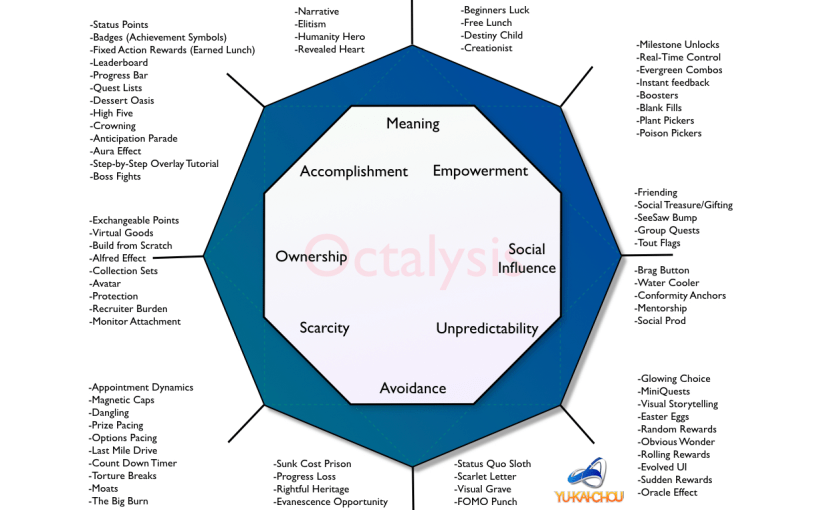
\includegraphics[width= 0.6\textwidth]{images/octaysis-gamification-framework.png}
    \end{center}
\end{itemize}

\subsection{The 8 Cor Drives of Gamification}
The following explanations are from Yu-Kai Chou's block (\url{https://yukaichou.com/gamification-examples/octalysis-complete-gamification-framework/}) and are more or less the same as described in his book.
\begin{itemize}
    \item \textbf{Core Drive 1: Epic Meaning \& Calling}
    \begin{center}
        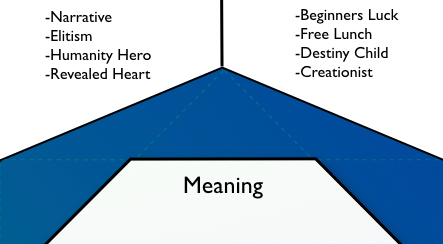
\includegraphics[width= 0.3\textwidth]{images/core-drive-1-epic-meaning-and-calling.png}
    \end{center}
    Epic Meaning \& Calling is the Core Drive where a player believes that he is doing something greater than himself or he was “chosen” to do something. A symptom of this is a player that devotes a lot of his time to maintaining a forum or helping to create things for the entire community (think Wikipedia or Open Source projects). This also comes into play when someone has “Beginner’s Luck” – an effect where people believe they have some type of gift that others don’t or believe they were “lucky” to get that amazing sword at the very beginning of the game.
    
    \item \textbf{Core Drive 2: Development \& Accomplishment}
    \begin{center}
        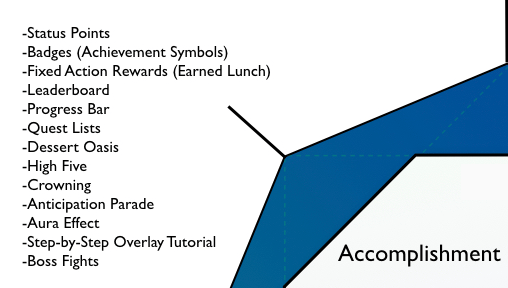
\includegraphics[width= 0.3\textwidth]{images/core-drive-2-development-and-accomplishment.png}
    \end{center}
    Development \& Accomplishment is the internal drive of making progress, developing skills, and eventually overcoming challenges. The word “challenge” here is very important, as a badge or trophy without a challenge is not meaningful at all. This is also the core drive that is the easiest to design for and coincidently is where most of the PBLs: points, badges, leaderboards mostly focus on.
    
    \item \textbf{Core Drive 3: Empowerment of Creativity \& Feedback}
    \begin{center}
        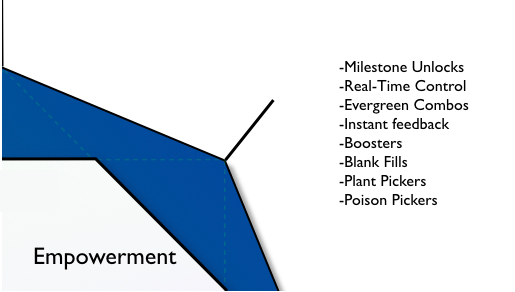
\includegraphics[width= 0.3\textwidth]{images/core-drive-3-empowerment-of-creativith-and-feedback.png}
    \end{center}
  Empowerment of Creativity \& Feedback is when users are engaged in a creative process where they have to repeatedly figure things out and try different combinations. People not only need ways to express their creativity, but they need to be able to see the results of their creativity, receive feedback, and respond in turn. This is why playing with Legos and painting are fun in-and-of themselves and often become Evergreen Mechanics, where a game-designer no longer needs to continuously add more content to keep the activity fresh and engaging.
  
      \item \textbf{Core Drive 4: Ownership \& Possession}
    \begin{center}
        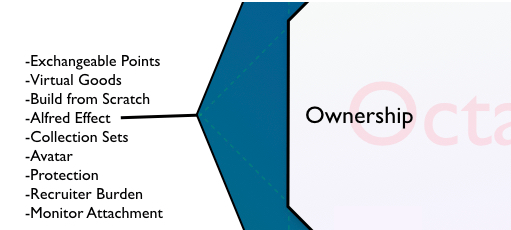
\includegraphics[width= 0.3\textwidth]{images/core-drive-4-ownership-and-possession.png}
    \end{center}
This is the drive where users are motivated because they feel like they own something. When a player feels ownership, she innately wants to make what she owns better and own even more. Besides being the major core drive for wanting to accumulate wealth, this deals with many virtual goods or virtual currencies within systems. Also, if a person spends a lot of time to customize her profile or her avatar, she automatically feels more ownership towards it too. Finally, this is also the core drive that makes collecting stamps or puzzle pieces fun.

      \item \textbf{Core Drive 5: Social Influence \& Relatedness}
    \begin{center}
        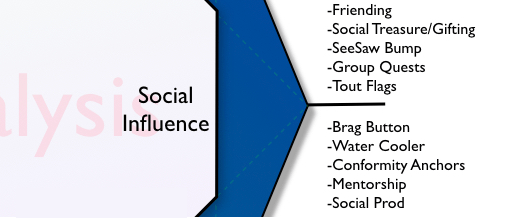
\includegraphics[width= 0.3\textwidth]{images/core-drive-5-social-influence-and-relatedness.png}
    \end{center}
This drive incorporates all the social elements that drive people, including: mentorship, acceptance, social responses, companionship, as well as competition and envy. When you see a friend that is amazing at some skill or owns something extraordinary, you become driven to reach the same level. Also, it includes the drive we have to draw closer to people, places, or events that we can relate to. If you see a product that reminds you of your childhood, the sense of nostalgia would likely increase the odds of you buying the product. This Core Drive is relatively well-studied too, as many companies these days are putting a lot of priority on optimizing their online social strategies.

      \item \textbf{Core Drive 6: Scarcity \& Impatience}
    \begin{center}
        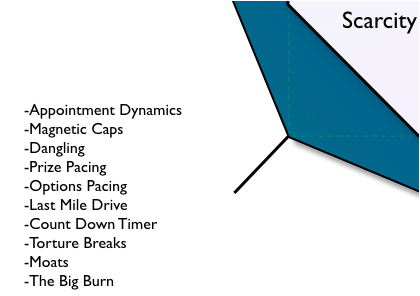
\includegraphics[width= 0.3\textwidth]{images/core-drive-6-scarcity-and-impatience.png}
    \end{center}
This is the drive of wanting something because you can’t have it. Many games have Appointment Dynamics (come back 2 hours later to get your reward) – the fact that people can’t get something right now motivates them to think about it all day long. This is the Core Drive utilized by Facebook when it first started: at first it was just for Harvard. Then it opened up to a few other prestigious schools, and eventually all colleges. When it finally opened up to everyone, many people wanted to join because they previously couldn’t get in it.

      \item \textbf{Core Drive 7: Unpredictability \& Curiosity}
    \begin{center}
        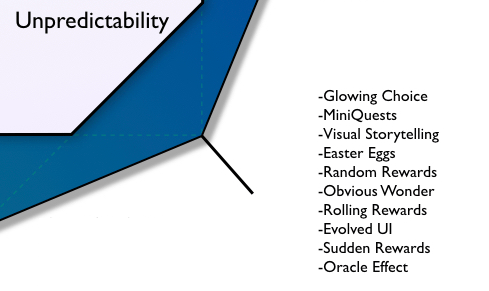
\includegraphics[width= 0.3\textwidth]{images/core-drive-7-unpredictability-and-curiosity.png}
    \end{center}
Generally, this is a harmless drive of wanting to find out what will happen next. If you don’t know what’s going to happen, your brain is engaged and you think about it often. Many people watch movies or read novels because of this drive. However, this drive is also the primary factor behind gambling addiction. Also, this core drive is utilized whenever a company runs a sweepstake or lottery program to engage users. The very controversial Skinner Box experiments, where an animal irrationally presses a lever frequently because of unpredictable results, are exclusively referring to the core drive of Unpredictability \& Curiosity, although many have misunderstood it as the driver behind points, badges, and leaderboard mechanics in general.

      \item \textbf{Core Drive 8: Loss \& Avoidance}
    \begin{center}
        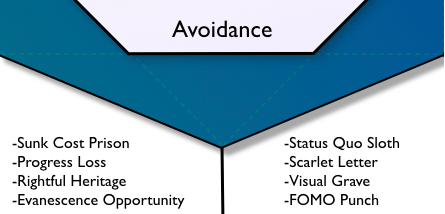
\includegraphics[width= 0.3\textwidth]{images/core-drive-8-loss-and-avoidance.png}
    \end{center}
This core drive is based upon the avoidance of something negative happening. On a small scale, it could be to avoid losing previous work. On a larger scale, it could be to avoid admitting that everything you did up to this point was useless because you are now quitting. Also, opportunities that are fading away have a strong utilization of this Core Drive, because people feel like if they didn’t act immediately, they would lose the opportunity to act forever.
\end{itemize}

\subsection{Left Brain vs. Right Brain}
\begin{center}
    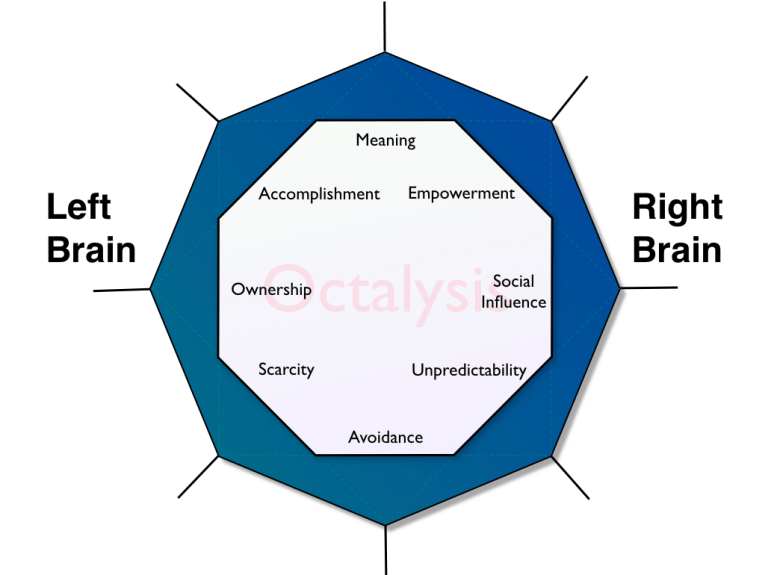
\includegraphics[width=0.6\textwidth]{images/left-brain-vs-right-brain-core-drives.png}
\end{center}
\begin{itemize}
    \item ''The Octalysis Framework is arranged so that the Core Drives that focus on creativity, self-expression, and social dynamics are organized on the right side of the octagon. In my framework I call them Right Brain Core Drives. The Core Drives that are most commonly associated with logic, analytical thought, and ownership are graphed on the left side of the octagon and are termed Left Brain Core Drives.''
\item ''Left Brain Core Drives tend to rely on Extrinsic motivation - you are motivated because you want to obtain something[..]. On the other hand, Right Brain Core Drives are mostly associated with Intrinsic Motivations - you don't need a goal or reward to use your creativity, hangout with friends, or feel the suspense of unpredictability - the activity itself is rewarding on its own.''
\item '' [M]any companies emphazise designing for Extrinsic Motivatiors, such as providing a reward when they complete a task. However, many studies have shown that extrinsic motivation impairs intrinsic motivation. Why? Because once the companies stop offering the extrinsic motivator, user motivation will often plummet to a level much lower than when the xtrinsic motivator was first introduced.''
\end{itemize}


\subsection{White Hat vs. Black Hat Gamification}
\begin{center}
    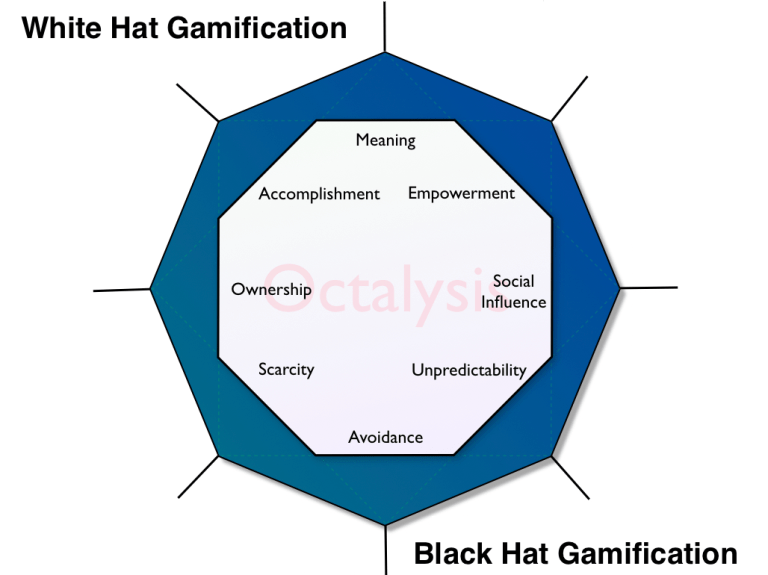
\includegraphics[width=0.6\textwidth]{images/white-hat-vs-black-hat-gamification.png}
\end{center}
''Another element to note within Octalysis is that the top Core Drives in the octagon are considered very positive motivators, while the bottom Core Drives are considered negative motivators.\\
\\
Techniques that utilize the top Core Drives are called “White Hat Gamification”,while techniques that utilize the bottom Core Drives are called “Black Hat Gamification”.\\
\\
If something is engaging because it lets you express your creativity, makes you feel successful through skill mastery, and gives you a higher sense of meaning, it makes users feel very good and powerful.\\
\\
On the other hand, if you are always doing something because you don’t know what will happen next, you are constantly in fear of losing something, or because there are things you can’t have, even though you would still be extremely motivated to take the actions, it can often leave a bad taste in your mouth.\\
\\
The problem with Zynga games [see \url{https://de.wikipedia.org/wiki/Zynga} for more information], according to the Octalysis framework, is that they have figured out how to do many Black Hat Game Techniques, which drive up revenue numbers from users, but it doesn’t make users feel good. So when a user is finally able to leave the system, they will want to, because they don’t feel like they are in control over themselves, just like gambling addiction.\\
\\
Keep in mind that just because something is Black Hat doesn’t mean it is necessarily bad – these are just motivators – and they can be used for productive and healthy results or malice and manipulative ones. Many people voluntarily submit themselves into Black Hat Gamification in order to go to the gym more often, eat healthy, or avoid hitting the snooze button every morning.\\
\\
A good Gamification expert will consider all 8 Core Drives on a positive and productive activity so that everyone ends up happier and healthier.'' (from his block)\\
\\
You are able to create an octagon for your personal application at \url{https://yukaichou.com/octalysis-tool/}

\subsection{Level 2 Octalysis Design for All 4 Phases}
\begin{itemize}
    \item There are more than 5 levels of the Octalysis design.
    \item ''Level 2 Octalysis, where we try to optimize experiences throughout all 4 phases of the player/user journey:
    \begin{enumerate}
        \item Discovery (why people would even want to try out the experience)
        \item Onboarding (where users learn the rules and tools to play the game)
        \item Scaffolding (the regular journey of repeated actions towards a goal)
        \item Endgame (how do you retrain your veterans)
    \end{enumerate}
    \item Most people treat their product as one experience, which seems reasonable. But in terms of motivation, I believe this is a mistake because the reason you are using a product on Day 1 is often very different from that of Day 100. Since everything you do is because of one of these Core Drives. If at any phase none of [them] is presented there is no reason for the user to move to the next phase.
    \item In the following ''illustration, you can evaluate how different Core Drives are more prominent during each Experience Phase[..].
    \begin{center}
            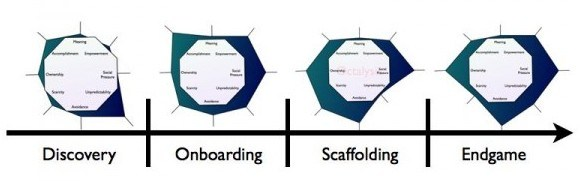
\includegraphics[width=0.6\textwidth]{images/Gamification-Octalysis.018-e1363796378415.jpg}
    \end{center}
\end{itemize}

\subsection{Level 3: Player Types}
\begin{center}
    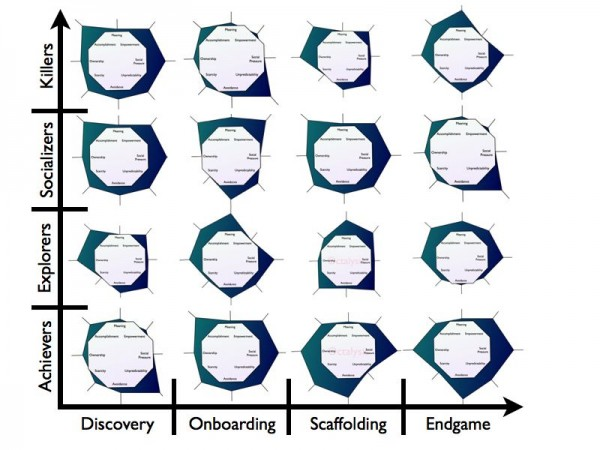
\includegraphics[width=0.5\textwidth]{images/Gamification-Octalysis.020.jpg}
\end{center}
\begin{itemize}
    \item In this diagram, Richard Bartle's Four Player Types are applied which is the most recognized model in game design.
    \item Bartle claims ''that is Four Player Types may not be suitable for gamification environments''.
    \item The point here is that different types of people are motivated differently, so Level 3 Octalysis allows the designer to understand and design for how everyone is feeling at different stages.''
    \item While there are five levels of Octalysis in total, Level 1 is often sufficient for the majority of companies seeking to understand why their products are not engaging their users. Higher-level Octalysis processes are useful for organizations that are truly commited to making sure that they push their metrics in the right direction and improve longevity of a gamified system.'' 
\end{itemize}